\chapter{Trace Encoder Output Packet}

The packets emerging from the encoder can be up to 35 bytes long
including 2 header bytes, an optional 2 byte timestamp and a variable
length payload. This can be seen in figure \ref{fig:packet-format}

\begin{figure}[h]
\begin{center}
  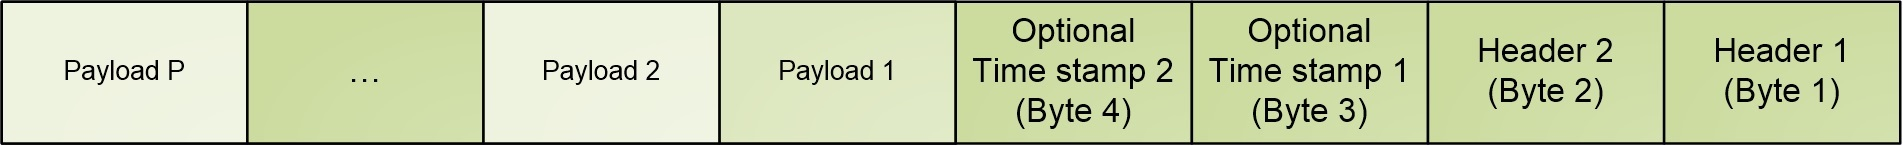
\includegraphics[height=1cm, width=9cm]{packet.jpg}
  \caption{Packet Format}
  \label{fig:packet-format}
\end{center}
\end{figure}


This packet format is used to output encoded instruction
trace.  Four different formats are used according to the needs of the
encoding algorithm. The following tables show the format of the
payload - i.e. not including the optional timestamp and not including
the the 2 byte header.

\begin{table}[htp]
    \centering
    \caption{Packet Format 0 and 1}
    \label{tab:te_inst0-1}
    \begin{tabulary}{\textwidth}{|l|p{35mm}|p{80mm}|}
        \hline
        {\bf Field name} & {\bf Bits} & {\bf Description} \\
        \hline
        \textbf{format}	& 2	& 00 (full-delta): includes branch map and full address \newline
                        01 (diff-delta): includes branch map and differential address\\
        \hline
        \textbf{branches} & 5 & Number of valid bits in branch-map. The length of branch-map is determined as follows: \newline
        0:      31 bits (\textbf{address} is not valid) \newline
        1: 	1 bit \newline
        2-9: 	9 bits \newline
        10-17: 	17 bits \newline
        18-25: 	25 bits \newline
        26-31: 	31 bits \newline
        For example if branches = 12, the branch-map is 17 bits long, and the 12 LSBs are valid. \newline
        In most cases when the branch map is full there is no need to report an address,
        and this is indicated by setting branches to 0.  The exception to this is when 
        the instruction immediately prior to the final branch causes an unpredictable discontinuity.\\
        \hline
        \textbf{branch-map} & Number of bits \newline 
                     determined by \newline 
                     \textbf {branches} field & 
                     An array of bits indicating whether branches are taken or not.\newline
        Bit 0 represents the oldest branch instruction executed.   For each bit: \newline
        0: branch taken \newline
        1: branch not taken \\
        \hline
        \textbf{address}	& Number of bits \newline 
                  is \textit {iaddress-width-p - iaddress-lsb-p} & 
                    Differential or full instruction address, according to \textbf {format}.  \newline
                    When branches is 0, the address is invalid, and is formed by sign extending branch-map.\\
        \hline
    \end{tabulary}
\end{table}


\begin{table}[!h]
    \centering
    \caption{Packet Format 2}
    \label{tab:te_inst2}
    \begin{tabulary}{\textwidth}{|l|p{35mm}|p{80mm}|}
        \hline
        {\bf Field name} & {\bf Bits} & {\bf Description} \\
        \hline
        \textbf{format}	& 2	& 10 (addr-only): address and no branch map\\
        \hline
        \textbf{address} & Total number of bits 
                  for address is
                  \textit {iaddress-width-p - iaddress-lsb-p}. & 
                  Address is always differential unless the encoder has been configured to only use full-address\\ 
        \hline
    \end{tabulary}
\end{table}

\begin{table}[htp]
    \centering
    \caption{Packet Format 3}
    \label{tab:te_inst3}
    \begin{tabulary}{\textwidth}{|l|p{35mm}|p{80mm}|}
      \hline
          {\bf Field name} & {\bf Bits} & {\bf Description} \\
          \hline
          \textbf{format} & 2 & 11 (sync): synchronisation\\
          \hline
          \textbf{subformat} & 2 & Sync sub-format omits fields when not required: \newline
          00 (start): ecause, interrupt and tval omitted \newline
          01 (exception): All fields present\newline
          10 (context): \textbf{address, branch, ecause, interrupt} and \textbf {tval} omitted \newline
          11 : reserved \\
          \hline
          \textbf{context} &  Total number of bits 
                     for context is  
                     \textit {context-width-p} 
                     unless  
                     \textit {nocontext-p} is 1,  
                     in which case it is 0 & 
                     The instruction context \\
          \hline
          \textbf{privilege} & Number of bits is  
                      \textit {privilege-width-p} & 
                      The current privilege level \\
          \hline
          \textbf{branch} & 1 & If the address points to a branch instruction, set to 1 if the branch was not taken. 
          Has no meaning if this instruction is not a branch. \\
          \hline
          \textbf{address} & number of bits is  
                    \textit {iaddress-width-p - iaddress-lsb-p},  
                    unless subformat is 10, & 
                    Full instruction address.  Address alignment is determined by \textit {iaddress-lsb-p} Address must be left shifted in order to recreate original byte address \\
          \hline
          \textbf{ecause} & Number of bits is  
                   \textit {ecause-width-p} if  
                   subformat is 01,  
                   or 0 otherwise  
                   (no exception). & 
                   Exception cause \\
          \hline
          \textbf{interrupt} & Number of bits is  
                      1 if subformat is 01,  
                      or 0 otherwise (no exception). & 
                      Interrupt \\
          \hline
          \textbf{tval} & Number of bits is  
                 \textit {iaddress-width-p}  
                 if subformat is  
                 01 and \textit {notval-p} is 
                 0, or 0 otherwise  
                 (no exception). & 
                 Trap value \\
          \hline
    \end{tabulary}
\end{table}

